\section{Fixing Boundary Imperfections\label{sec:precision}}%: Aggregation v.s. Retrieval Comparison}
% \subsection{Retrieval-based methods}
% This class of algorithms tries to identify good and bad workers, and then chooses the best worker segmentation as the output segmentation. In this paper, we look at two different ways of ranking workers and choosing the best worker. First, we use the {\em number of control points}, i.e. number of vertices in a worker's segmentation polygon to rank workers. This is a ranking scheme that~\cite{Vittayakorn2011} showed performs well in practice. Intuitively, workers that have used a larger number of points are likely to have been more precise, and provided a more complex and accurate segmentation. Other heuristic ranking scheme is described in more detail in our technical report~\cite{segmentation-tr}.
\begin{figure}[h!]
\vspace{-10pt}
\centering
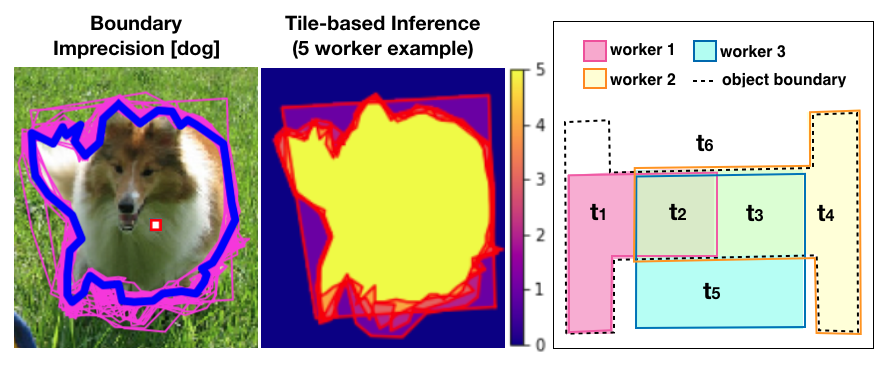
\includegraphics[width=0.8\textwidth]{plots/precision_issue_tile_example.png}
\caption{Left: Pink boundaries shows worker segmentations and blue delineates the ground truth. Right: Segmentation boundaries drawn by five workers shown in red. Overlaid segmentation creates a masks where the color indicates the number of workers who voted for the tile region.}
\label{tile_demo}
\end{figure}
% \vspace{-10pt}
At the heart of our aggregation techniques is the ``tile'' data representation, where we logically overlay all workers' segmentations on top of each other, as illustrated in Figure \ref{tile_demo} right, to create non-overlapping discrete tile units. The intuition here is that by splitting the image into tiles, we get finer granularity information than by looking at complete segmentations. This also allows us to aggregate data from multiple workers rather than having to choose a single worker bounding box---enabling the opportunity to choose partial segmentations by fixing one worker's errors via the help from another worker's segmentation.
% Now, we will describe several algorithms for picking a good set of tiles.
The goal of our aggregation algorithms, described below, is to pick a good set of tiles that effectively trade-off precision versus recall.

\stitle{Aggregation: Majority Vote Aggregation (MV)} 
\par \noindent Include a tile in the output segmentation if and only if the tile is covered by at least 50\% of all worker segmentations.

\stitle{Aggregation: Expectation-Maximization (EM)}
\par \noindent Unlike MV, which assumes that all workers performs uniformly, EM approaches use worker quality models to infer the likelihood that a tile is part of the ground truth segmentation. The EM algorithm simultaneously estimate both worker qualities and tile likelihoods as hidden variables. Details of the formal derivation and three worker quality models that we have developed can be found in our technical report.

\stitle{Aggregation: Greedy Tile Picking (greedy)} 
\par \noindent The greedy algorithm sorts tiles in descending order based on their overlap area to non-overlap area ratio, and then picks tiles in that order, effectively picking tiles in order of their contribution to the jaccard similarity against ground truth, for as long as the estimated jaccard of the resulting segmentation continue to increase. The challenge here is that tile overlap and non-overlap areas are not known, so we use a number of heuristics, including the tile probabilities from EM to estimate these areas. Furthermore, we cannot compute the actual jaccard score against the hidden ground truth, so we use a heuristic baseline like the MV segmentation as a proxy for the ground truth.

\stitle{Retrieval: Number of Control Points (num pts)}
\par \noindent Pick the worker segmentation with the largest number of control points around the segmentation boundary (i.e. most precise drawing) as the output segmentation.